\documentclass[unknownkeysallowed]{beamer}
\usepackage[french,english]{babel}
\usepackage{../sty/beamer_js}
\usepackage{../sty/shortcuts_js}

\definecolor{tomcolor}{rgb}{0.,.3,.6}
\lstset{basicstyle=\color{tomcolor}\scriptsize\ttfamily}
\addbibresource{../biblio/biblio.bib}

\begin{document}

%%%%%%%%%%%%%%%%%%%%%%%%%%%%%%%%%%%%%%%%%%%%%%%%%%%%%%%%%%%%%%%%%%%%%%%%%%%%%%%
%%%%%%%%%%%%%%%%%%%%%%             Headers               %%%%%%%%%%%%%%%%%%%%%%
%%%%%%%%%%%%%%%%%%%%%%%%%%%%%%%%%%%%%%%%%%%%%%%%%%%%%%%%%%%%%%%%%%%%%%%%%%%%%%%


%%%%%%%%%%%%%%%%%%%%%%%%%%%%%%%%%%%%%%%%%%%%%%%%%%%%%%%%%%%%%%%%%%%%%%%%%%%%%%%
\begin{frame}
\bigskip
\bigskip
\begin{center}{
\LARGE\color{marron}
\textbf{Benchopt:\\
		Benchmarking optimization Algorithms}
\textbf{ }\\
\vspace{0.5cm}
}

\color{marron}
% \textbf{or... an introduction to Beamer instead}
\end{center}

\vspace{0.5cm}

\begin{center}
\textbf{Joseph Salmon} \\
\vspace{0.1cm}
\url{http://josephsalmon.eu}\\
\vspace{0.5cm}
Université de Montpellier \\
\end{center}

\centering

\includegraphics[width=0.13\textwidth]{um_logo}

\end{frame}
%%%%%%%%%%%%%%%%%%%%%%%%%%%%%%%%%%%%%%%%%%%%%%%%%%%%%%%%%%%%%%%%%%%%%%%%%%%%%%%



%%%%%%%%%%%%%%%%%%%%%%%%%%%%%%%%%%%%%%%%%%%%%%%%%%%%%%%%%%%%%%%%%%%%%%%%%%%%%%%
%%%%%%%%%%%%%%%%%%%%%%%%       RoadMap   %%%%%%%%%%%%%%%%%%%%%%%%%%%%%%%%%%%%%%
%%%%%%%%%%%%%%%%%%%%%%%%%%%%%%%%%%%%%%%%%%%%%%%%%%%%%%%%%%%%%%%%%%%%%%%%%%%%%%%


% % Uncomment for table of content
% %%%%%%%%%%%%%%%%%%%%%%%%%%%%%%%%%%%%%%%%%%%%%%%%%%%%%%%%%%%%%%%%%%%%%%%%%%%%%%%
% \begin{frame}{Table of Contents}
% \tableofcontents[hideallsubsections]
% \end{frame}
% %%%%%%%%%%%%%%%%%%%%%%%%%%%%%%%%%%%%%%%%%%%%%%%%%%%%%%%%%%%%%%%%%%%%%%%%%%%%%%%


% %%%%%%%%%%%%%%%%%%%%%%%%%%%%%%%%%%%%%%%%%%%%%%%%%%%%%%%%%%%%%%%%%%%%%%%%%%%%%%%
% \AtBeginSection[]
% {
% \begin{frame}<beamer>{Table of Contents}
% \tableofcontents[currentsubsection,
%     hideothersubsections,
%     sectionstyle=show/shaded,
% ]
% \end{frame}
% }
% %%%%%%%%%%%%%%%%%%%%%%%%%%%%%%%%%%%%%%%%%%%%%%%%%%%%%%%%%%%%%%%%%%%%%%%%%%%%%%%



%%%%%%%%%%%%%%%%%%%%%%%%%%%%%%%%%%%%%%%%%%%%%%%%%%%%%%%%%%%%%%%%%%%%%%%%%%%%%%%
\begin{frame}{Benchmarking algorithms in practice}

Choosing the best algorithm to solve an optimization problem often depends on:\\[1em]

\begin{minipage}{.8\textwidth}
\begin{itemize}
	\item The data \mybold{scale, conditionning}
	\item The objective parameters \mybold{regularisation}
	\item The implementation \mybold{complexity, language}
\end{itemize}
\end{minipage}

\vskip2em
An impartial selection requires a time consuming {\bf benchmark}!\\[1em]


The goal of {\bf Benchopt} is to make this step as easy as possible.

\end{frame}
%%%%%%%%%%%%%%%%%%%%%%%%%%%%%%%%%%%%%%%%%%%%%%%%%%%%%%%%%%%%%%%%%%%%%%%%%%%%%%%



%%%%%%%%%%%%%%%%%%%%%%%%%%%%%%%%%%%%%%%%%%%%%%%%%%%%%%%%%%%%%%%%%%%%%%%%%%%%%%%
\begin{frame}[fragile]{Benchopt}

Doing a  benchmark for the $\ell_2$ regularized logistic regression with multiple solvers and datasets is now easy as calling:\\[1em]

% \begin{beamercolorbox}[shadow=true, wd=.96\textwidth, sep=.2em, rounded=true]{title}

    % \textcolor[rgb]{0,.3,.6}{
\begin{lstlisting}[language=bash]
git clone https://github.com/benchopt/benchmark_logreg_l2
benchopt run ./benchmark_logreg_l2
\end{lstlisting}
% \end{beamercolorbox}

\vskip1.5em
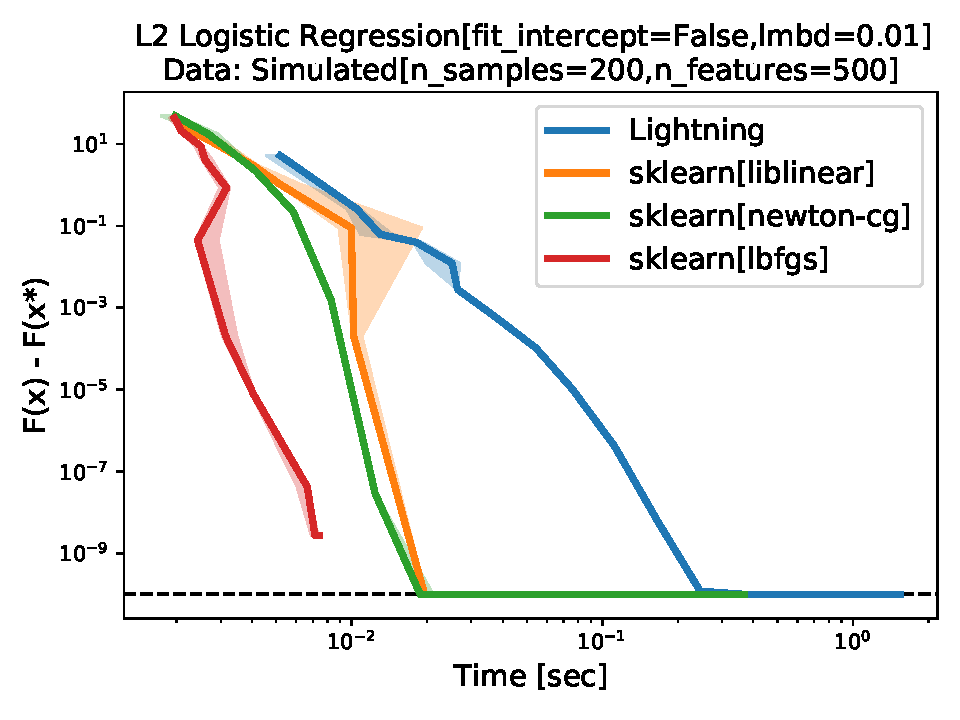
\includegraphics[width=.45\textwidth]{logreg_l2}
\hskip3ex
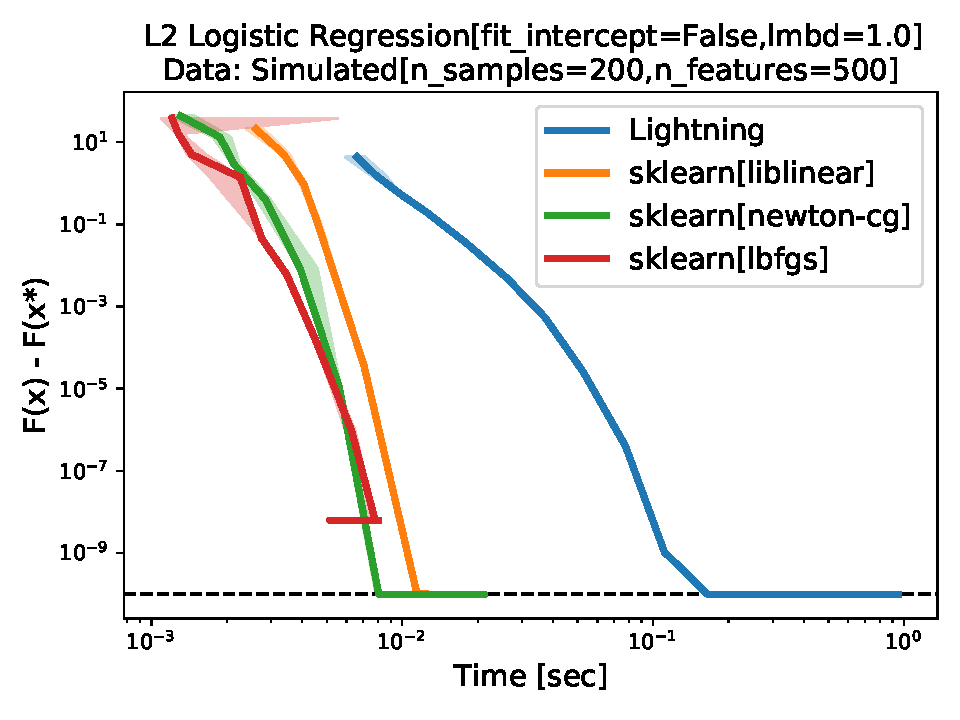
\includegraphics[width=.45\textwidth]{logreg_l2_1}

\end{frame}
%%%%%%%%%%%%%%%%%%%%%%%%%%%%%%%%%%%%%%%%%%%%%%%%%%%%%%%%%%%%%%%%%%%%%%%%%%%%%%%


%%%%%%%%%%%%%%%%%%%%%%%%%%%%%%%%%%%%%%%%%%%%%%%%%%%%%%%%%%%%%%%%%%%%%%%%%%%%%%%
\begin{frame}{Benchopt}

Benchopt can also compare the same algo in different languages.\\[1em]

Here is an example comparing PGD in: Python; R; Julia.\\[1em]
{\centering
\vskip.5em
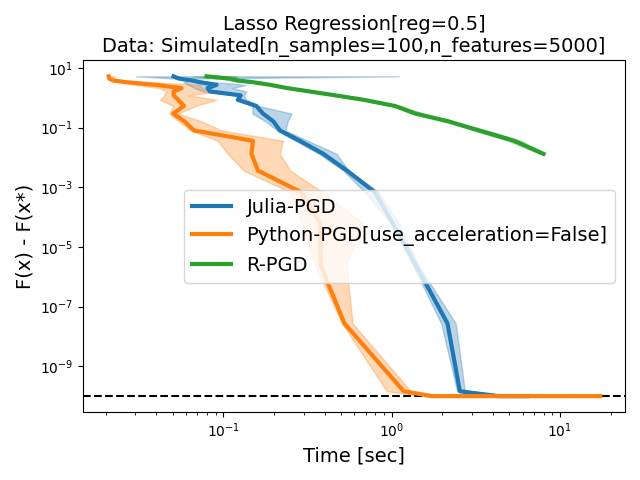
\includegraphics[width=.65\textwidth]{lasso_3_languages}\\}

\end{frame}
%%%%%%%%%%%%%%%%%%%%%%%%%%%%%%%%%%%%%%%%%%%%%%%%%%%%%%%%%%%%%%%%%%%%%%%%%%%%%%%


%%%%%%%%%%%%%%%%%%%%%%%%%%%%%%%%%%%%%%%%%%%%%%%%%%%%%%%%%%%%%%%%%%%%%%%%%%%%%%%
\begin{frame}{Benchmark: principle}

A benchmark is a directory with:\\
\begin{itemize}
    \item An \lstinline+objective.py+ file with an \lstinline+Objective+,
    \item A directory \lstinline+solvers+ with one file per \lstinline+Solver+,
    \item A directory \lstinline+datasets+ with \lstinline+Dataset+ generators/fetchers.
\end{itemize}
\vskip1em
Each of these objects can be parametrized.\\

The \lstinline+benchopt+ client runs a cross product and generates a csv file + convergence plots like above.\\[.5em]
We expose easy way to select the \lstinline+objective/solver/dataset+ you want to run.
\end{frame}
%%%%%%%%%%%%%%%%%%%%%%%%%%%%%%%%%%%%%%%%%%%%%%%%%%%%%%%%%%%%%%%%%%%%%%%%%%%%%%%


%%%%%%%%%%%%%%%%%%%%%%%%%%%%%%%%%%%%%%%%%%%%%%%%%%%%%%%%%%%%%%%%%%%%%%%%%%%%%%%
\begin{frame}{Benchmarks}

So far, we have implemented benchmarks for:\\[.5em]
\begin{itemize}
	\item Least Square
	\item Non-Negative Least Square
	\item Lasso
	\item L1/L2 Regularized Logistic Regression
\end{itemize}

\vskip1em
Feel free to join our effort to create reproducible benchmarks by adding new objectives/solvers/datasets!!!\\[1em]

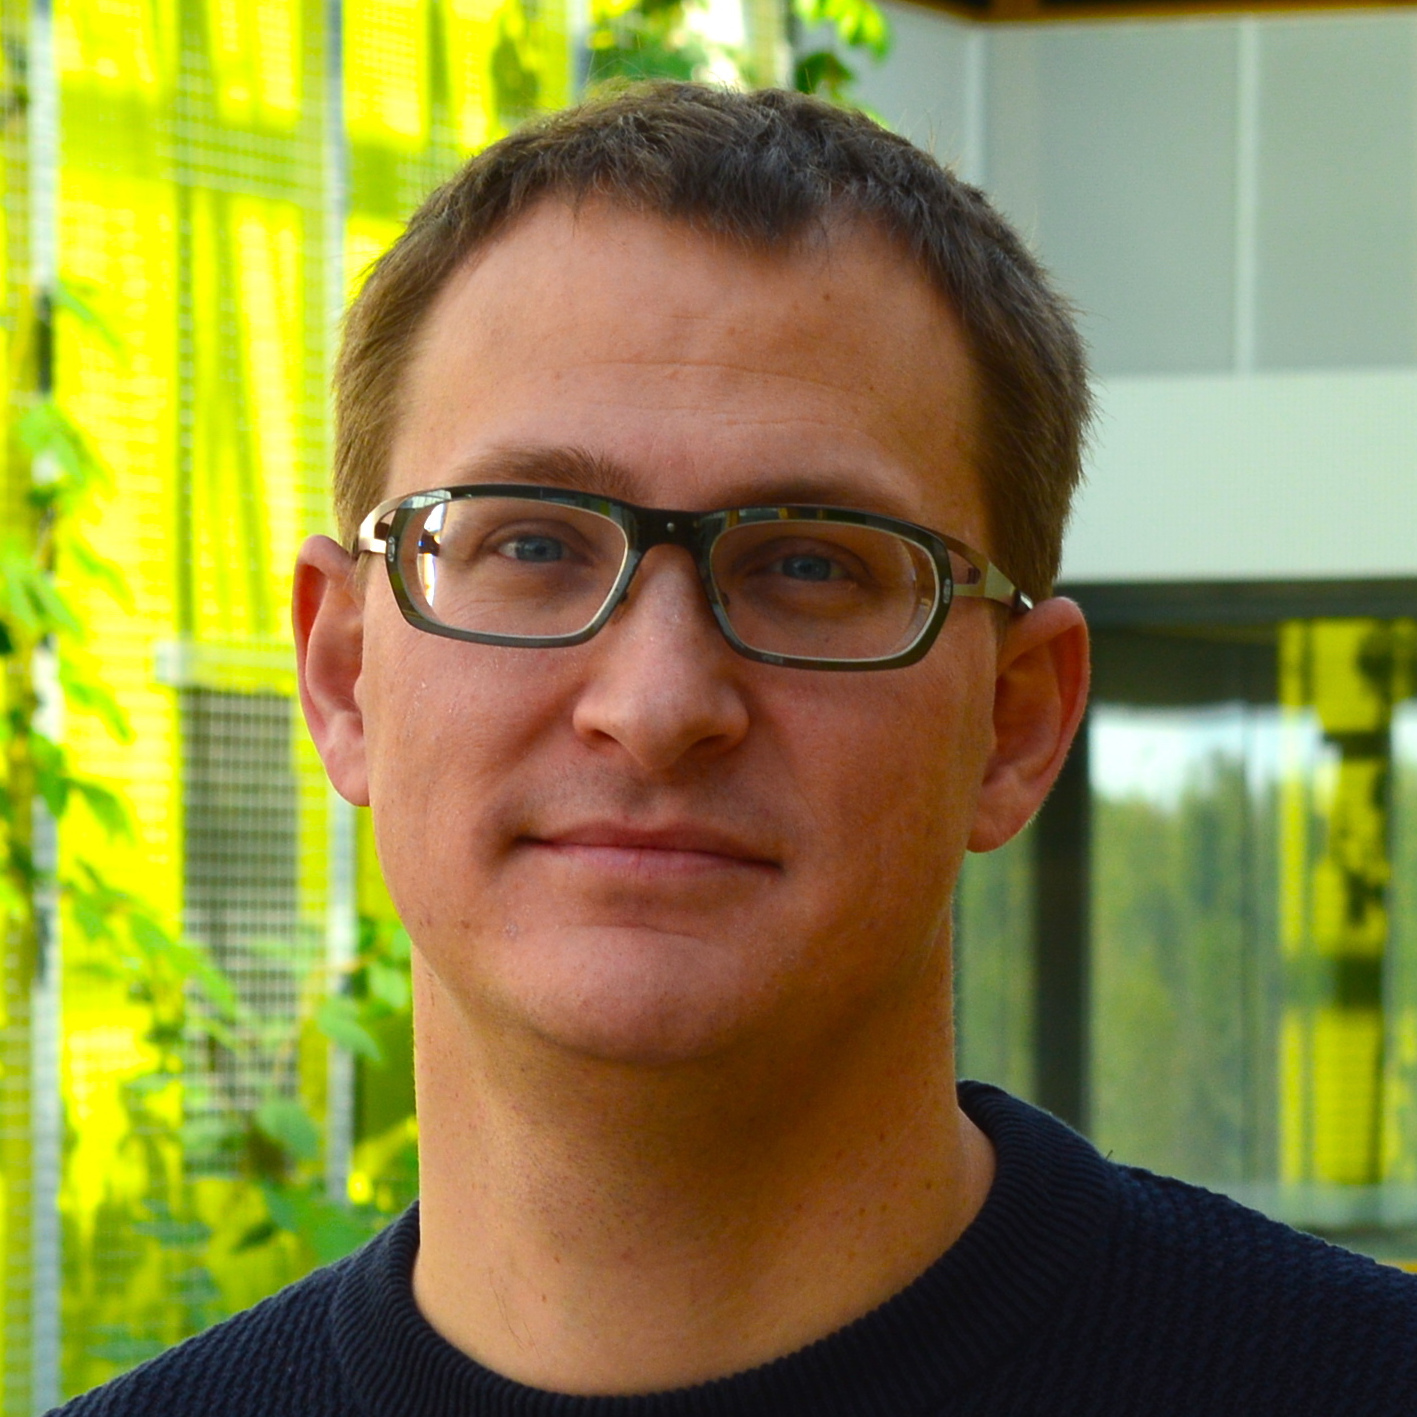
\includegraphics[width=.19\textwidth]{agramfort}
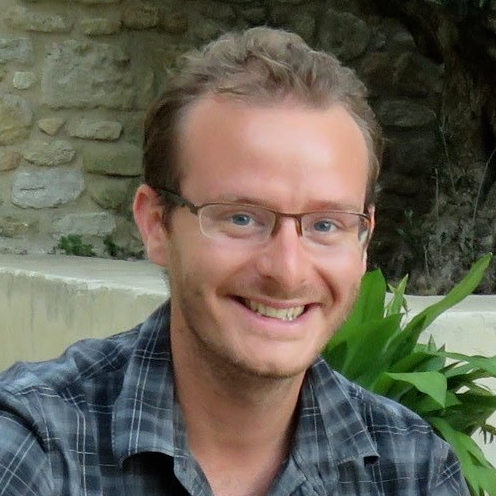
\includegraphics[width=.19\textwidth]{jsalmon}
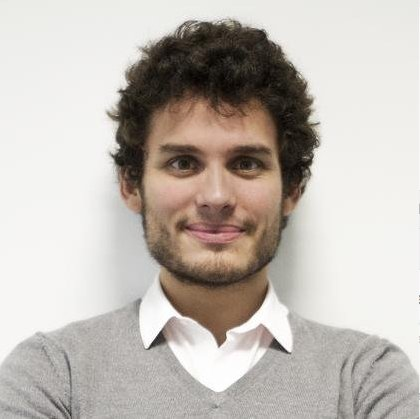
\includegraphics[width=.19\textwidth]{mmassias}
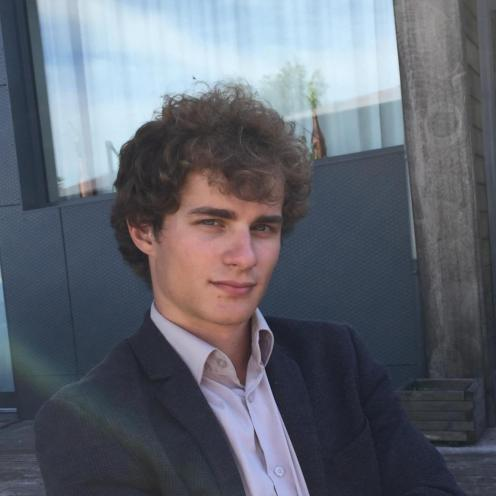
\includegraphics[width=.19\textwidth]{tomdlt}

\includegraphics[width=.19\textwidth]{tommoral}

\end{frame}
%%%%%%%%%%%%%%%%%%%%%%%%%%%%%%%%%%%%%%%%%%%%%%%%%%%%%%%%%%%%%%%%%%%%%%%%%%%%%%%


%%%%%%%%%%%%%%%%%%%%%%%%%%%%%%%%%%%%%%%%%%%%%%%%%%%%%%%%%%%%%%%%%%%%%%%%%%%%%%%
\begin{frame}{Benchopt}
    \centering
    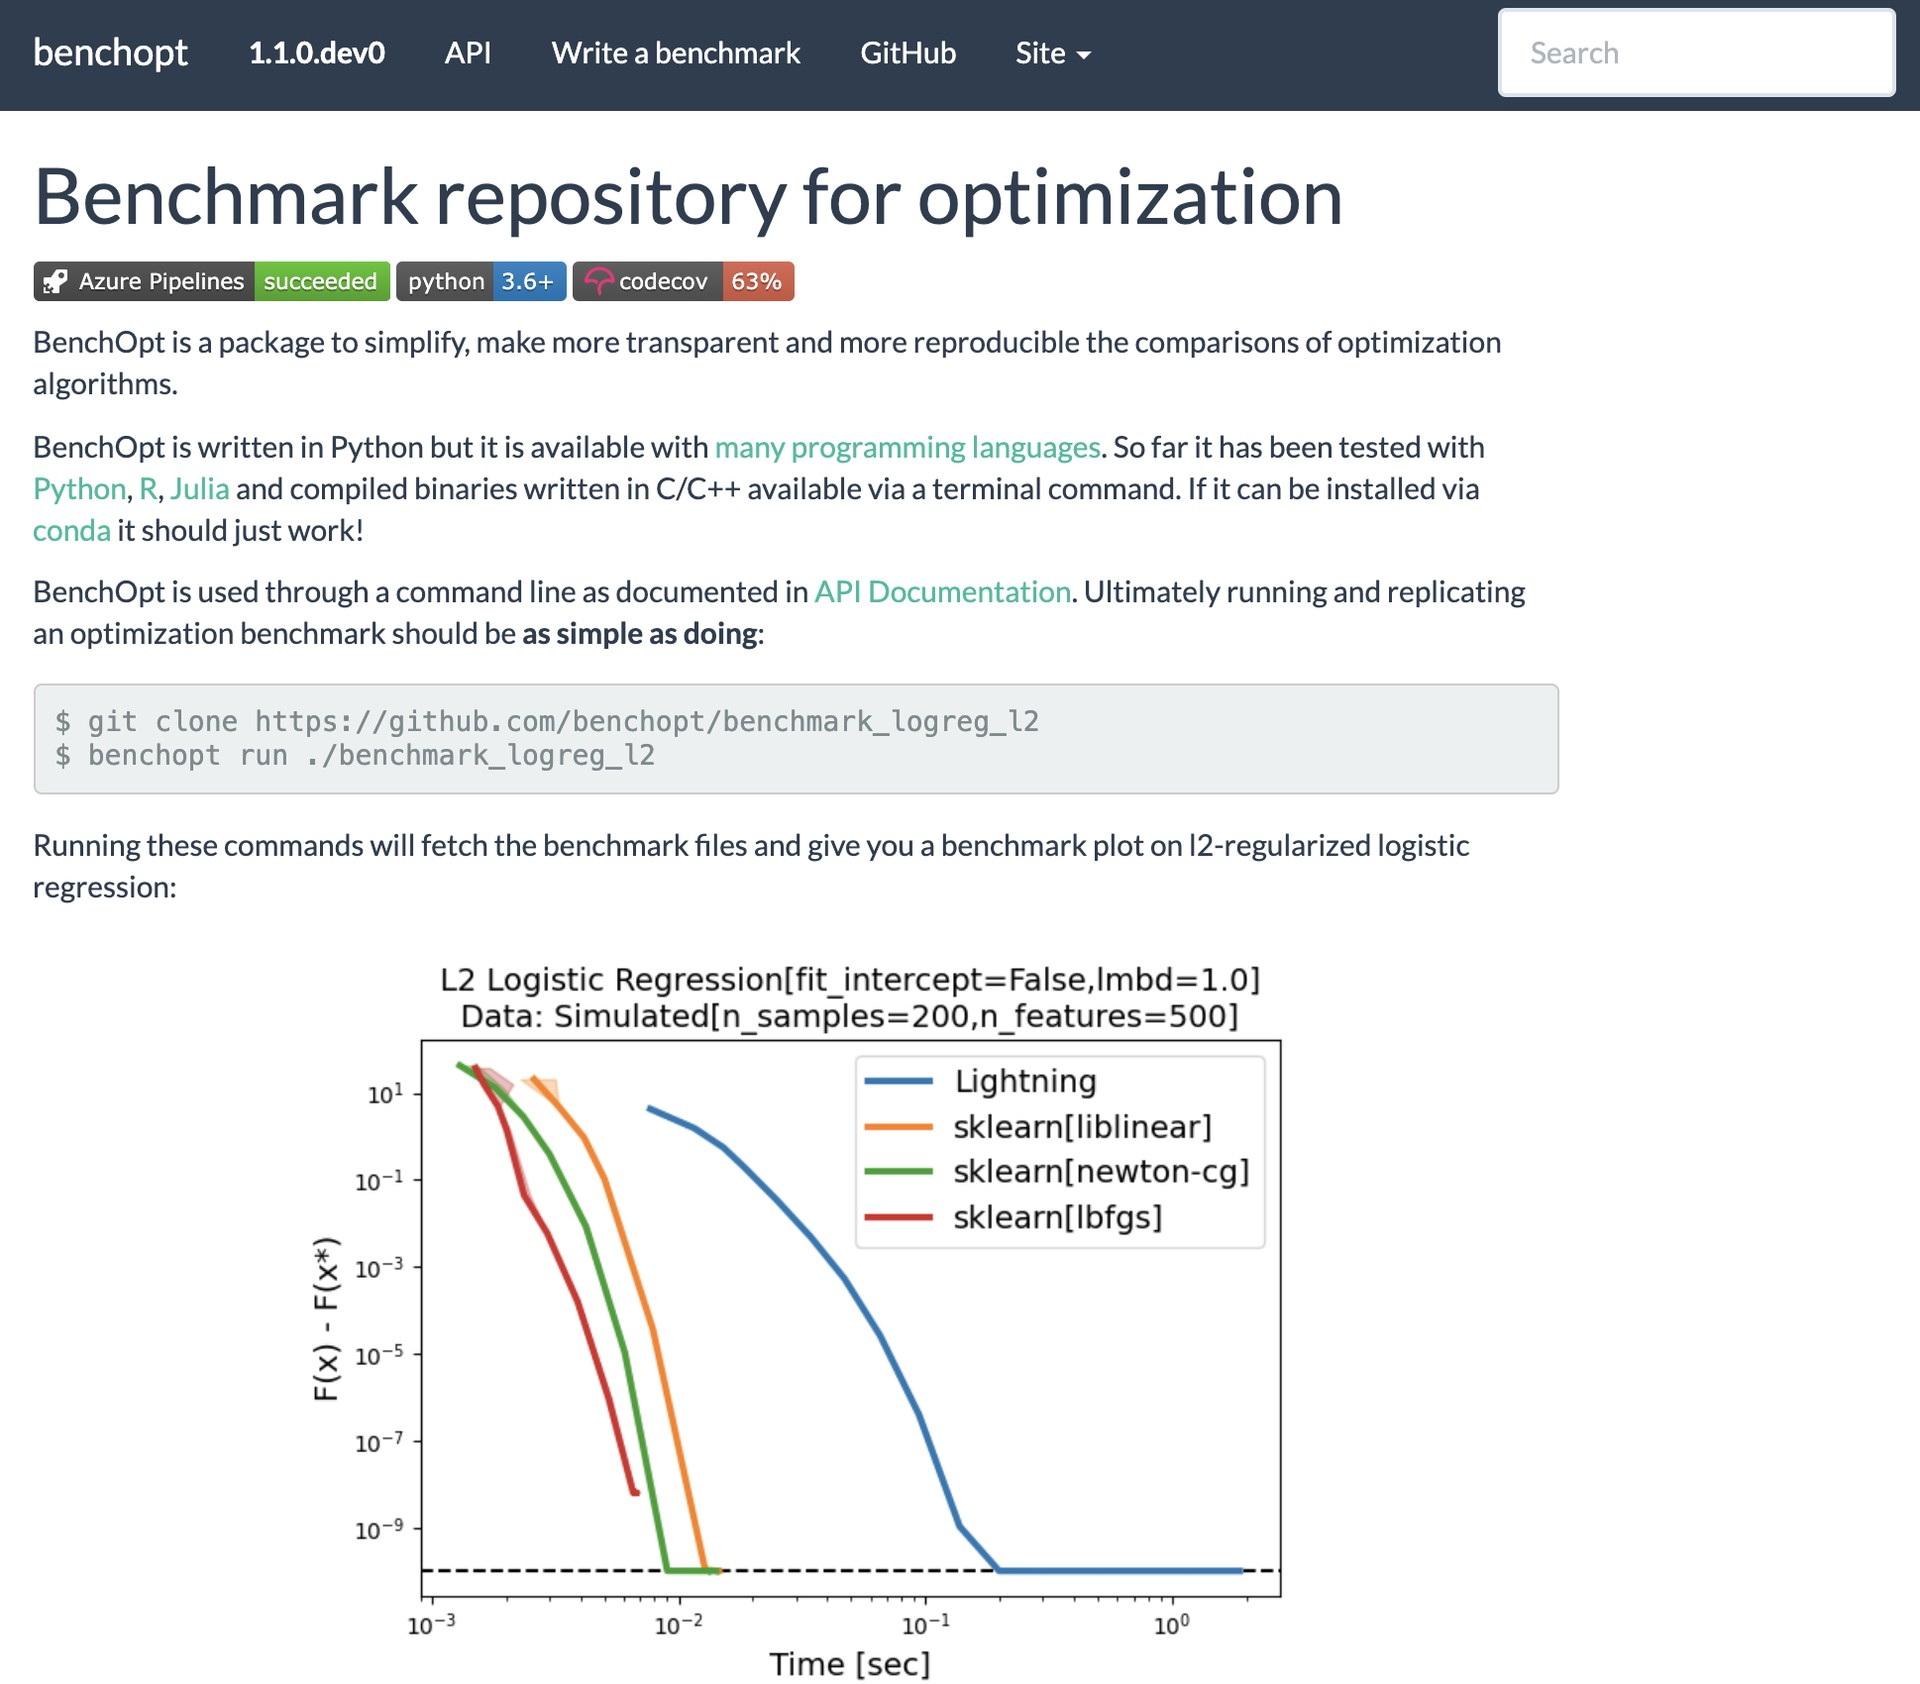
\includegraphics[width=.9\textwidth]{benchopt}\\
\end{frame}
%%%%%%%%%%%%%%%%%%%%%%%%%%%%%%%%%%%%%%%%%%%%%%%%%%%%%%%%%%%%%%%%%%%%%%%%%%%%%%%


%%%%%%%%%%%%%%%%%%%%%%%%%%%%%%%%%%%%%%%%%%%%%%%%%%%%%%%%%%%%%%%%%%%%%%%%%%%%%%%
\begin{frame}{Contact}

\vspace{0.4cm}
\centering

\includegraphics[width=0.93\textwidth]{contact_js}
\end{frame}
%%%%%%%%%%%%%%%%%%%%%%%%%%%%%%%%%%%%%%%%%%%%%%%%%%%%%%%%%%%%%%%%%%%%%%%%%%%%%%%



% %%%%%%%%%%%%%%%%%%%%%%%%%%%%%%%%%%%%%%%%%%%%%%%%%%%%%%%%%%%%%%%%%%%%%%%%%%%%%%%
% % Uncomment for references
% \begin{frame}{Bibliographie}
% \printbibliography
% \end{frame}
%  %%%%%%%%%%%%%%%%%%%%%%%%%%%%%%%%%%%%%%%%%%%%%%%%%%%%%%%%%%%%%%%%%%%%%%%%%%%%%%



\end{document}
